
%----------------------------------------------------------------------------------------
%	Settings and packages
%----------------------------------------------------------------------------------------

\documentclass[10pt]{article}

\usepackage{colortbl}
\usepackage{multirow}
\usepackage[table]{xcolor}
\usepackage{ctable}
\usepackage{float}
\usepackage[landscape,margin=0.25in,legalpaper]{geometry}

\newcommand{\mcn}[2]{\multicolumn{#1}{l}{#2}}	
\newcommand{\mccn}[2]{\multicolumn{#1}{c}{#2}}
\newcommand{\mcl}[1]{\multicolumn{2}{l}{#1}}
\newcommand{\mclg}[1]{\multicolumn{2}{l}{\gr #1}}
\newcommand{\mcc}[1]{\multicolumn{2}{c}{#1}}
\newcommand{\mccg}[1]{\multicolumn{2}{c}{\gr #1}}
\newcommand{\mr}[1]{\multirow{-2}{*}{#1}}
\definecolor{Gray}{gray}{0.90}
\newcommand{\gr}{\cellcolor{Gray}}

\newcommand{\thickline}{\specialrule{.1em}{.05em}{.05em}}

\setlength\parindent{0pt}

% column colours
\newcolumntype{g}{>{\columncolor{Gray}}l}
\newcolumntype{w}{>{\columncolor{white}}l}

%----------------------------------------------------------------------------------------
%	Create new commands
%----------------------------------------------------------------------------------------

% Commands are in LatexCommands.tex. New commands for this file only can be written here.
%\input{/Applications/TeX/Latex_ancillary/LatexCommands.tex}


%----------------------------------------------------------------------------------------
%	Table
%----------------------------------------------------------------------------------------

\begin{document}

\thispagestyle{empty}
{\bf 2008 Deepwell Cup}
\begin{table}[h!]
    \centering
    \begin{tabular}{l g g w w g g w w g g w w}
        \rowcolor{black}\mcn{13}{\color{white}\bf Round 3: Conference Finals} \\
        \rowcolor{white}\\
        &  \mccg{Andrew D}&  \mcc{Daniel S}&  \mccg{David D}&  \mcc{Kollin H}&  \mccg{Michael D}&  \mcc{Thomas L} \\\thickline
        {\bf East} &&&&&&&&&&&&\\\hline
          Pittsburgh Penguins&&&&&&&&&&&&\\
          Philadelphia Flyers & \mr{PIT} & \mr{7} & \mr{PIT} & \mr{6} & \mr{PHI} & \mr{6} & \mr{PIT} & \mr{6} & \mr{PHI} & \mr{6} & \mr{PIT} & \mr{7}\\\hline
          &&&&&&&&&&&& \\
        {\bf West} &&&&&&&&&&&&\\\hline
          Detroit Red Wings&&&&&&&&&&&&\\
          Dallas Stars & \mr{DAL} & \mr{7} & \mr{DET} & \mr{5} & \mr{DAL} & \mr{6} & \mr{DET} & \mr{6} & \mr{DAL} & \mr{6} & \mr{DET} & \mr{6}\\\hline
          \rowcolor{white}\\
        \rowcolor{black} \mcn{13}{\color{white}\bf Conference Champions} \\
          Eastern & \mclg{MTL} & \mcl{MTL} & \mclg{MTL} & \mcl{MTL} & \mclg{MTL} & \mcl{MTL}\\
          Western & \mclg{DET} & \mcl{SJS} & \mclg{ANA} & \mcl{SJS} & \mclg{SJS} & \mcl{ANA}\\
          Stanley Cup & DET & 6 & MTL & 7 & MTL & 6 & SJS & 7 & SJS & 6 & MTL & 6
    \end{tabular}
\end{table}

{\bf Points}\\
\begin{minipage}{12cm}
    \begin{tabular}{l l}
        Correct team:	& $7$\\
        Correct series length (regardless of series winner):	& $10$\\
        Stanley Cup champion (in addition to finalist):	& 10\\
        Stanley Cup finalist:	& 15\\
    \end{tabular}

    \vspace{1cm}
    {\bf Number of picks per team:}\\
    \begin{tabular}{lc | lc }
        PIT & 4 & DET & 3 \\
        PHI & 2 & DAL & 3 \\
    \end{tabular}
\end{minipage}
\begin{minipage}[t]{13cm}
    \begin{figure}[H]
        \vspace{-2.5cm}
        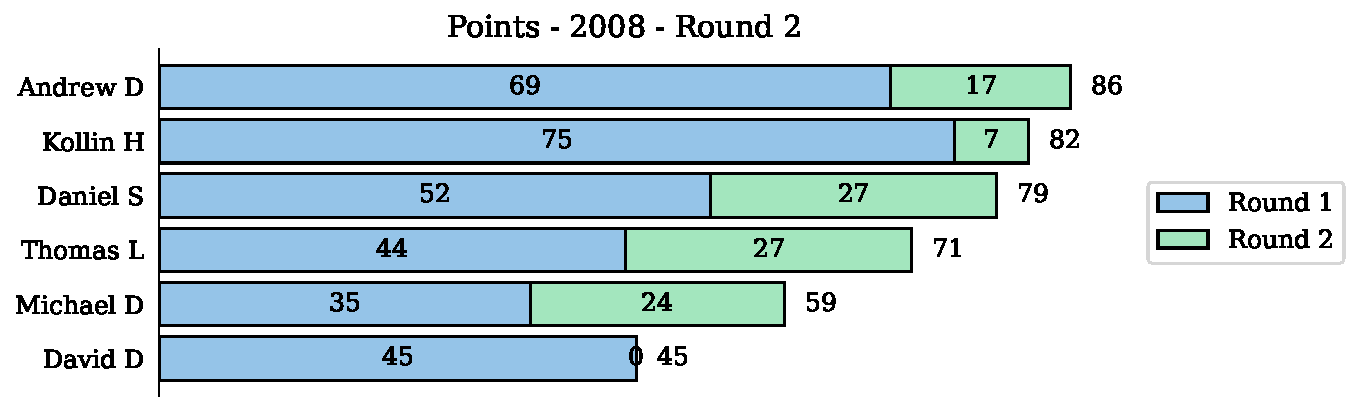
\includegraphics[width=13cm]{../../figures/2008/Points-2008-Round2.pdf}
    \end{figure}
\end{minipage}

\end{document}